%!TeX program = xelatex
%Do not change
\documentclass[12pt, oneside]{article}
\usepackage{amssymb,amsmath}
\usepackage[margin=1in]{geometry}
\usepackage{textpos}
\usepackage{float}
%\usepackage{color}
\usepackage{graphicx}
\usepackage[inter-unit-product =\cdot]{siunitx}
%\usepackage{tikz}
%\usetikzlibrary{positioning}
%\usepackage{tikz-3dplot}
%\usepackage{pgfopts}
%\usepackage{wasysym}
%\usepackage{stanli}

% You may add the packages you need here
\begin{document}

%TODO change numbers in problems
\begin{textblock*}{4cm}(-1.7cm,-2.3cm)
\noindent {\scriptsize AE333 Fall 2020}
\end{textblock*}

%Do not modify other than putting your name where stated
\begin{textblock*}{8cm}(12.5cm,-1cm)
\noindent {Name: }
\end{textblock*}
%Do not modify other than typing your acknowledgement where stated
\begin{textblock*}{13.5cm}(-1.7cm,-1.8cm)
%\noindent \textit{\footnotesize Acknowledgement: Your acknowledgement for collaboration and other sources goes here. }
\end{textblock*}

\vspace{1cm}

%Do not modify other than typing the homework number after #
\begin{center}
\textbf{\Large Homework 1}

\textbf{Due 25 Aug 2020}
\end{center}

%Rest should contain your solution for the homework. Feel free to improvise in ways that you believe make grading easier.
\begin{enumerate}
	\item %1-16
		Find the internal load at points D and E.
		\begin{figure}[H]
			\centering
			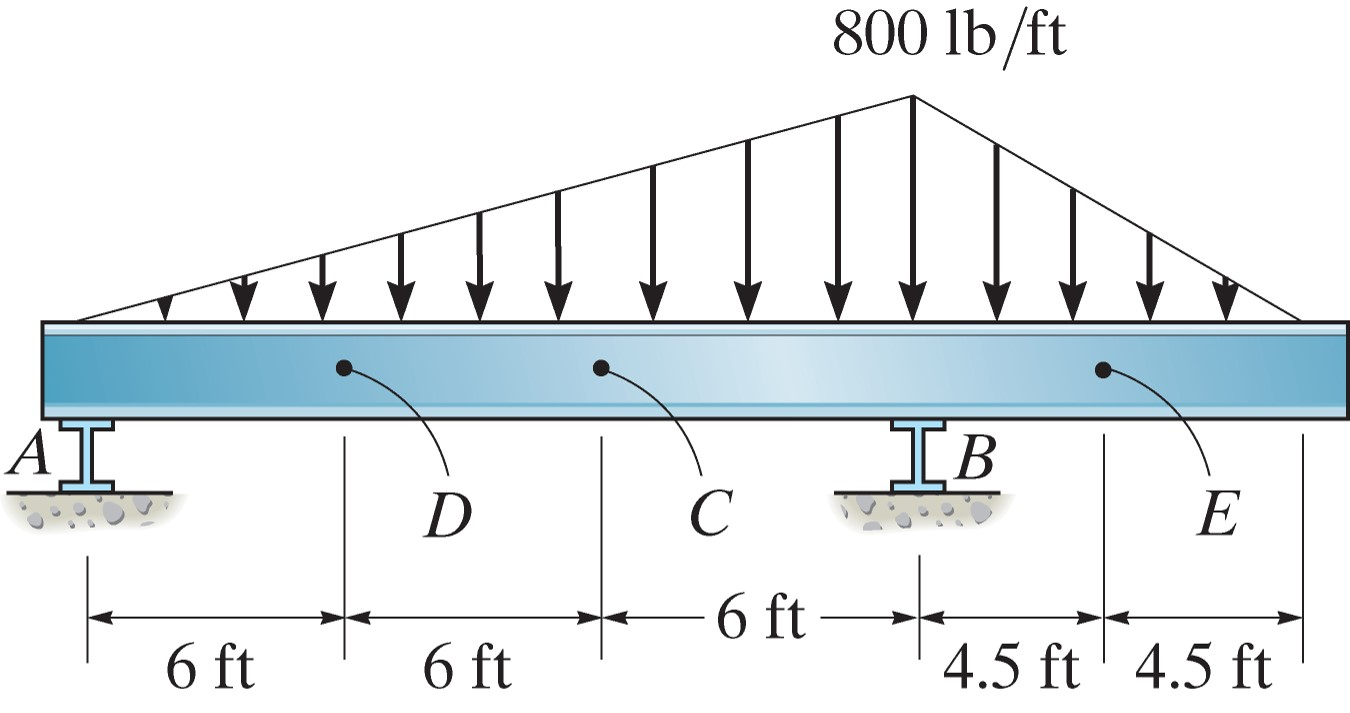
\includegraphics[width=0.6\linewidth]{beam}
			\label{fig:beam}
		\end{figure}
	
	\item %1-14
		A hacksaw (and many other styles of thin-bladed saws) are held stiff via a pretensioning as shown.
		For a pre-load force of 120 N, find the internal loading acting on section $b-b$ through point $D$.
		\begin{figure}[H]
			\centering
			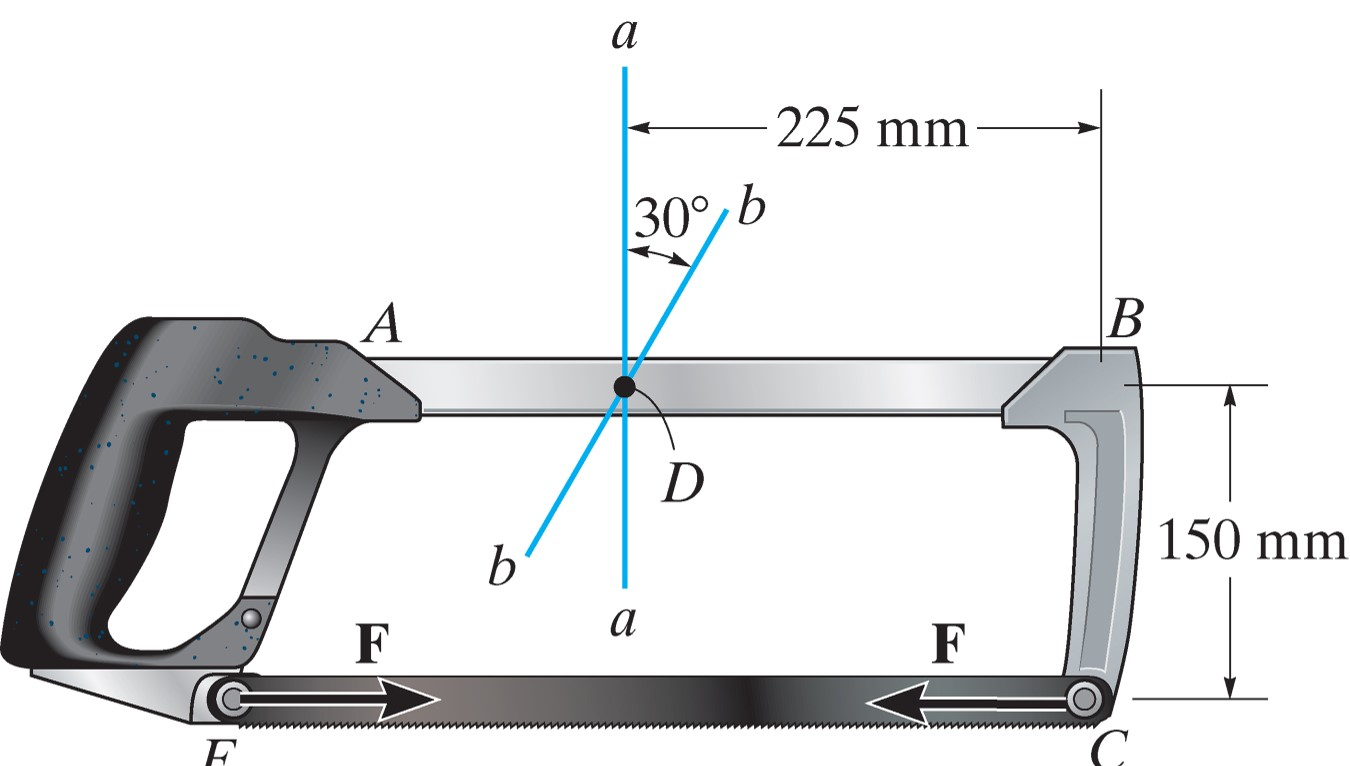
\includegraphics[width=0.6\linewidth]{hacksaw}
			\label{fig:hacksaw}
		\end{figure}
		\pagebreak

	\item %1-28
		A bit brace is a type of hand drill.
		If the brace shown jams and is subjected to the force shown, find the resultant internal loading on the shank of the drill bit (point A).
		\begin{figure}[H]
			\centering
			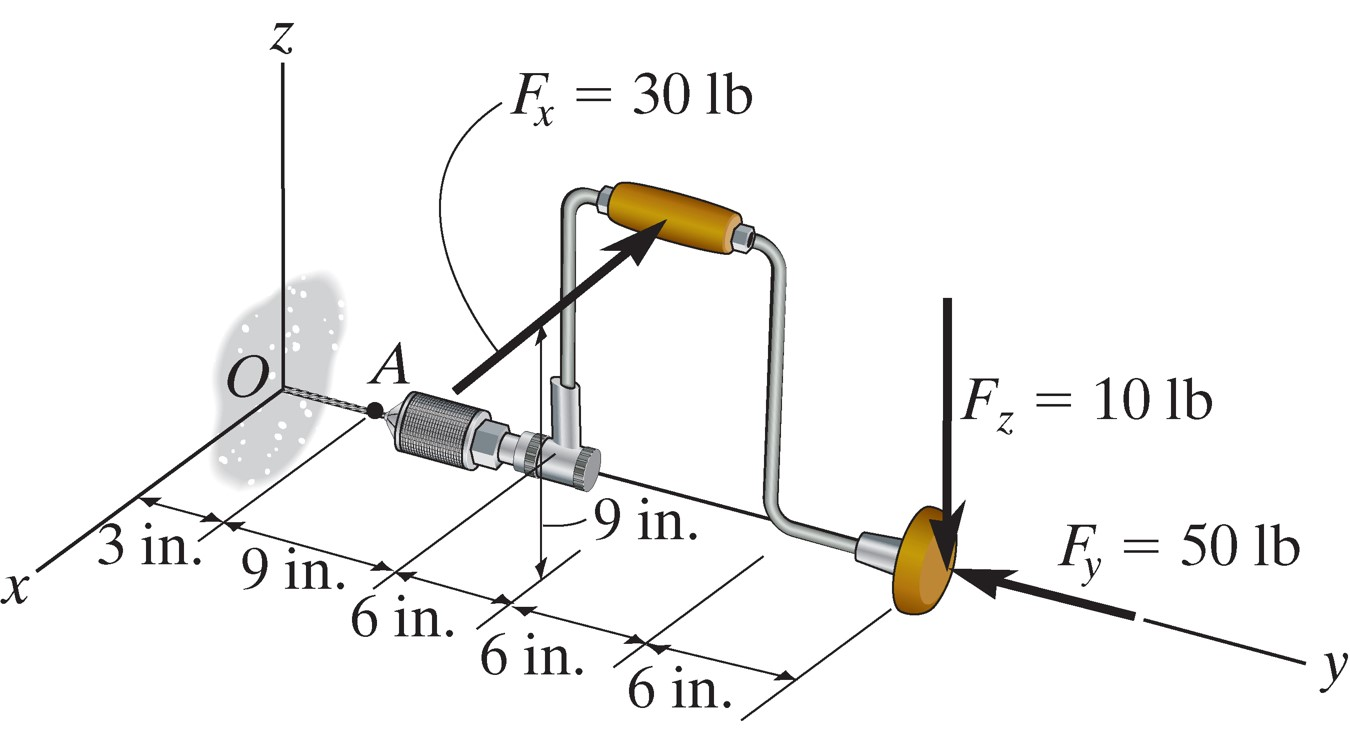
\includegraphics[width=0.6\linewidth]{brace}
			\label{fig:brace}
		\end{figure}

	\item %1-32
		Determine the largest uniform load, $w$, that can be applied to the frame shown without exceeding an average tensile stress of $\sigma = \SI{15}{MPa}$ or an average shear stress of $\tau = \SI{16}{MPA}$ along section $b-b$.
		The bars shown are square tubes $\SI{40}{mm}$ on the outside and $\SI{30}{mm}$ on the inside.
		\begin{figure}[H]
			\centering
			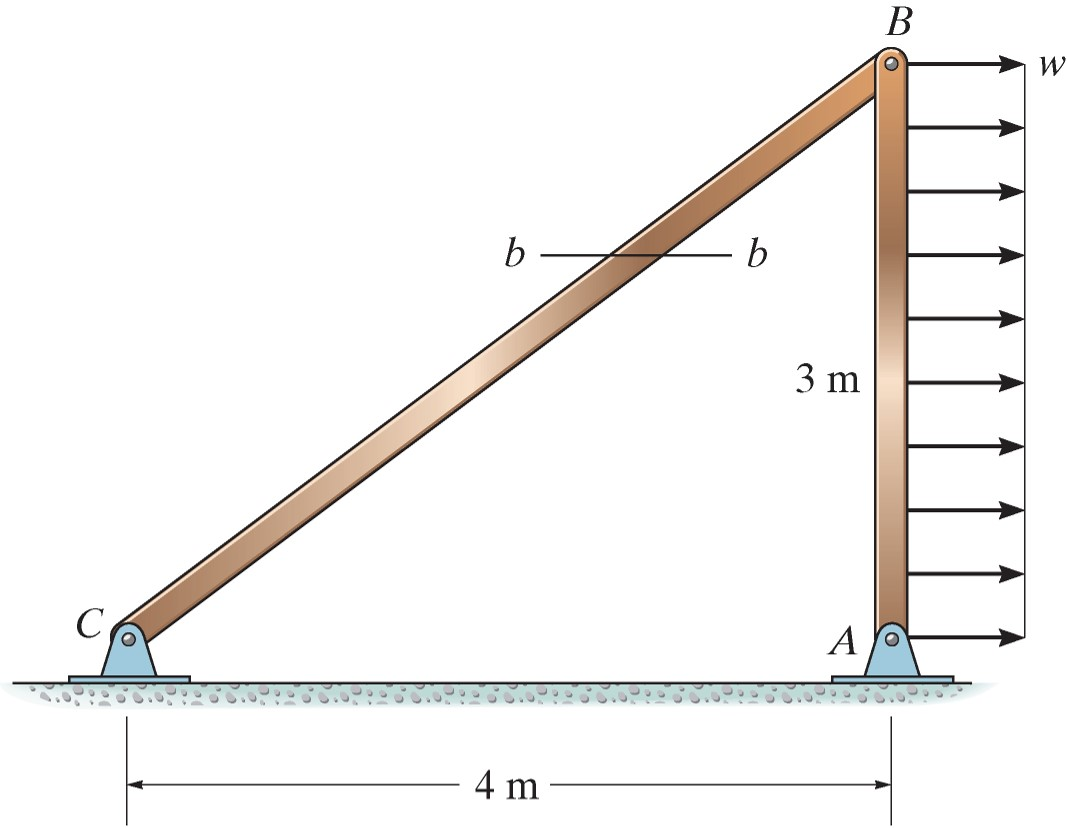
\includegraphics[width=0.6\linewidth]{truss}
			\label{fig:truss}
		\end{figure}
		\pagebreak
	
	\item %1-54
		Two members for an airframe are welded together using a $30^\circ$ fish-mouth weld.
		Find the average shear stress on the plane of each weld for the case shown.
		\begin{figure}[H]
			\centering
			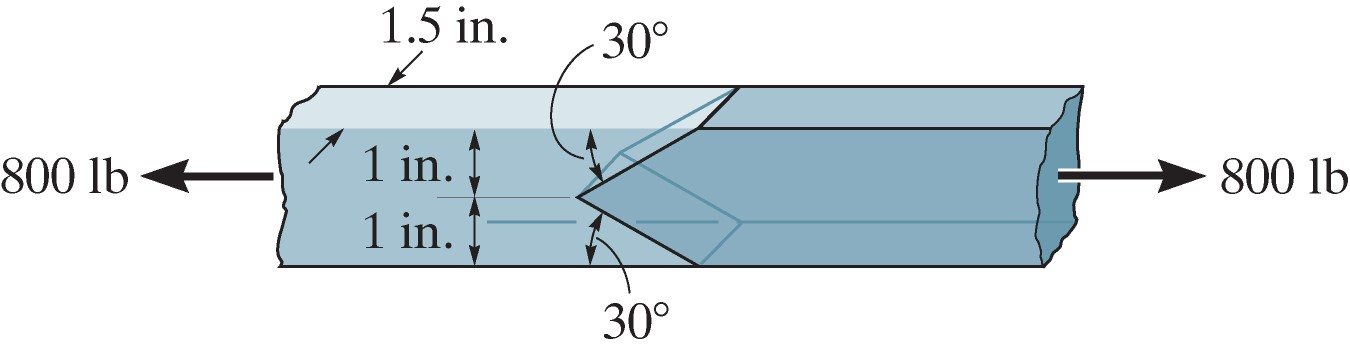
\includegraphics[width=0.6\linewidth]{fish-mouth}
			\label{fig:fish-mouth}
		\end{figure}

	\item %1-86
		Two aluminum rods support a vertical force of $P=\SI{20}{kN}$.
		Find the diameter of the rods (they are solid and have the same diameter) for a failure stress of $\sigma=\SI{120}{MPa}$ and a safety factor of 1.5.
		\begin{figure}[H]
			\centering
			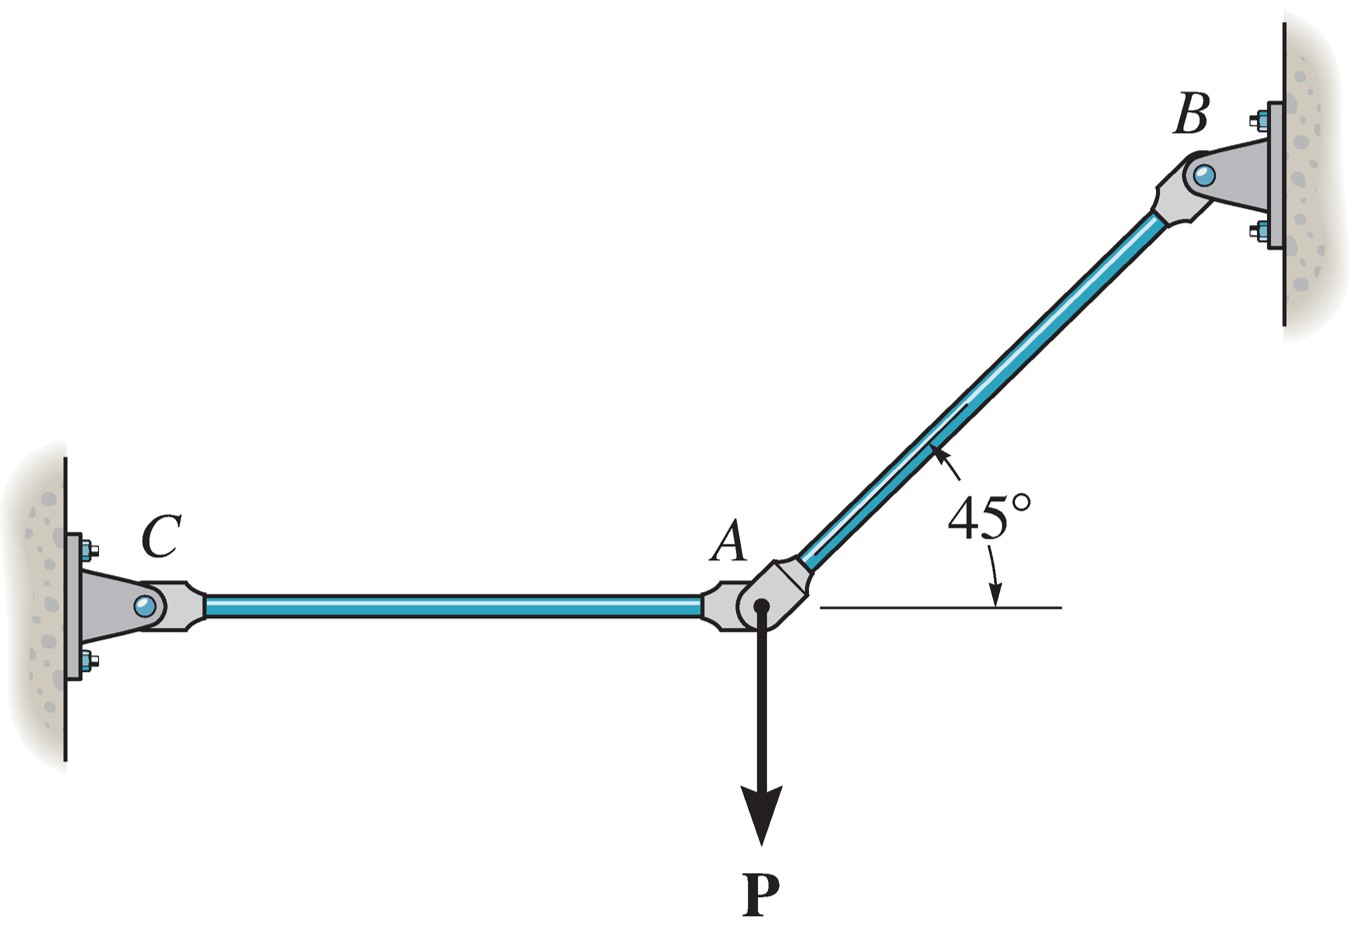
\includegraphics[width=0.6\linewidth]{rods}
			\label{fig:rods}
		\end{figure}
		\pagebreak

	\item %1-93
		The two rods ($AB$ and $CD$) supporting beam $AC$ are made of steel.
		Determine the smallest rod diameter to support the dead loads shown along with an additional live load of $\SI{5}{kN}$.
		The resistance factor for steel in tension is $\phi=0.9$, use a dead load factor of $\gamma_D = 1.4$ and a live load factor of $\gamma_L = 1.9$.
		The failure stress for this steel alloy is $\sigma_{fail} = \SI{360}{MPa}$.
		\begin{figure}[H]
			\centering
			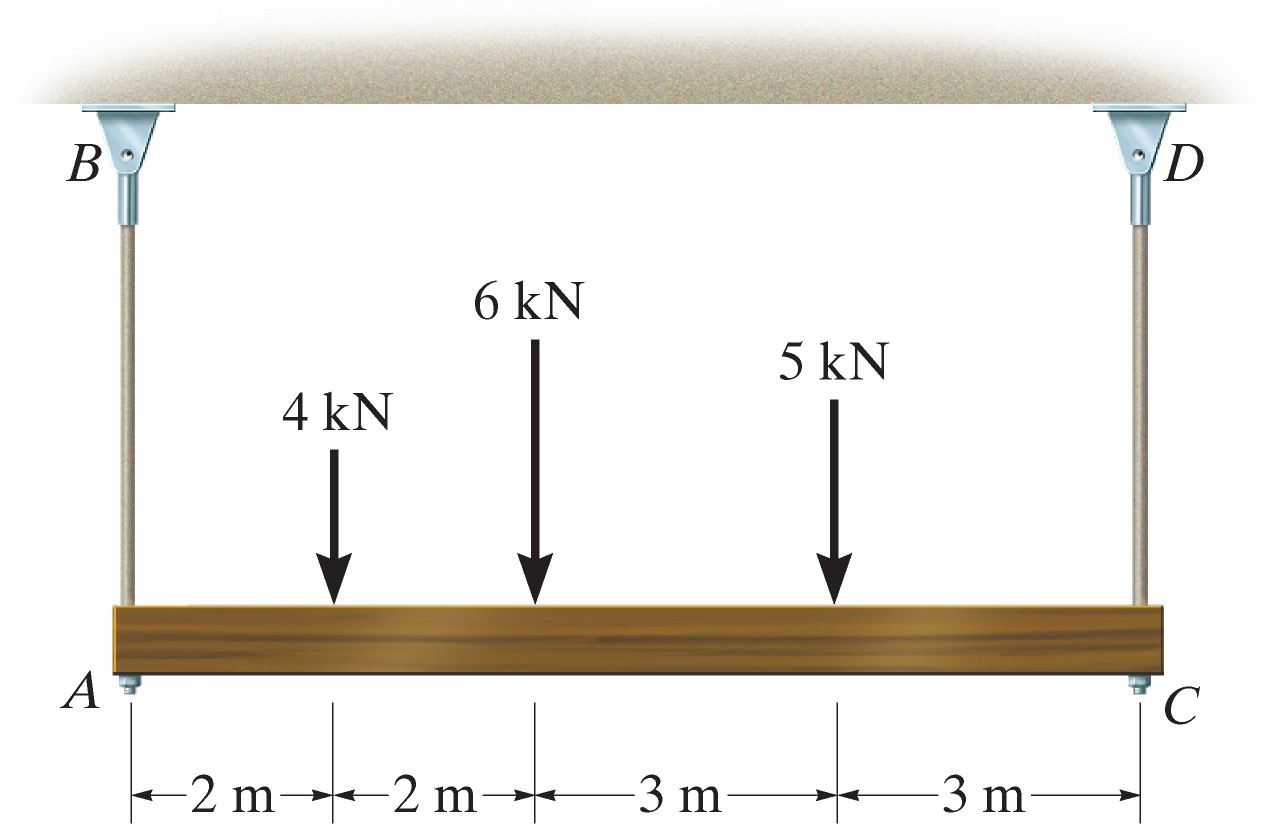
\includegraphics[width=0.6\linewidth]{hangingbeam}
			\label{fig:hangingbeam}
		\end{figure}

	\item %C1-1
		Extreme high winds can cause failure of highway signs, as shown here.
		Assuming a uniform wind pressure of $\SI{3}{kPa}$, estimate reasonable sign dimensions and determine the resultant shear where the failure occurred.
		Compare your answer with the material properties listed on the back cover of your textbook (or an online database), does this seem like a reasonable failure or do you suspect some bad assumptions?
		\begin{figure}[H]
			\centering
			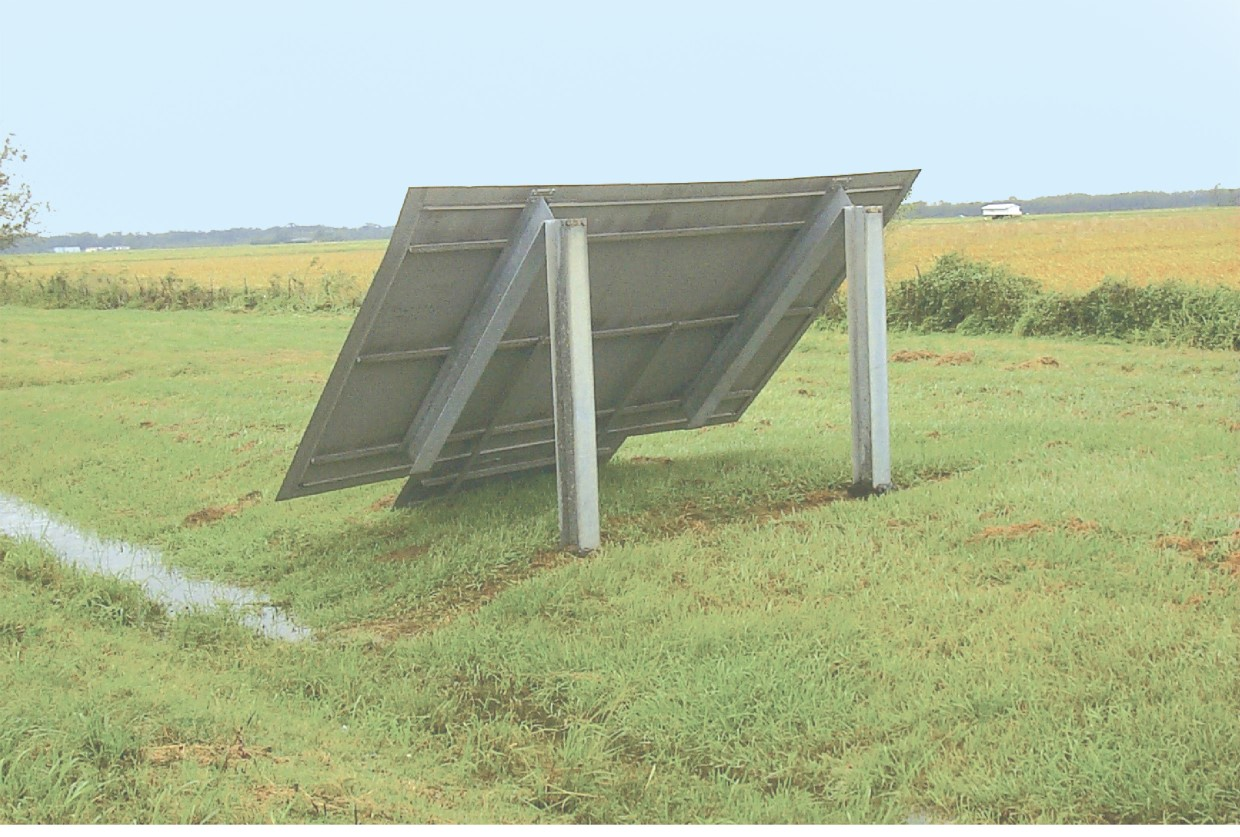
\includegraphics[width=0.6\linewidth]{sign}
			\label{fig:sign}
		\end{figure}
		\pagebreak

	\item %C1-3
		The bolt shown has failed due to single shear.
		Use free body diagrams to show why the bolt failed at this point and not somewhere else.
		\begin{figure}[H]
			\centering
			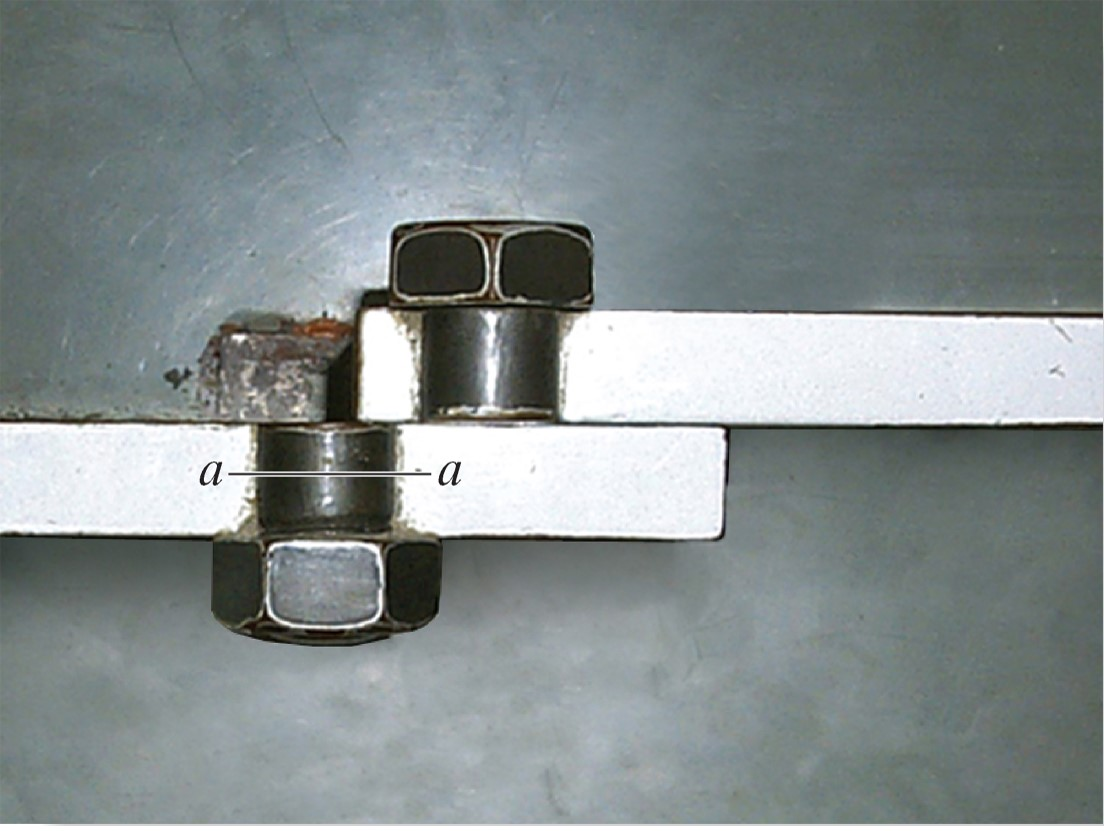
\includegraphics[width=0.6\linewidth]{bolt}
			\label{fig:bolt}
		\end{figure}

\end{enumerate}
\end{document}
